\chapter{Schematics and layout}

  \begin{figure}[h]
	  \centering
	  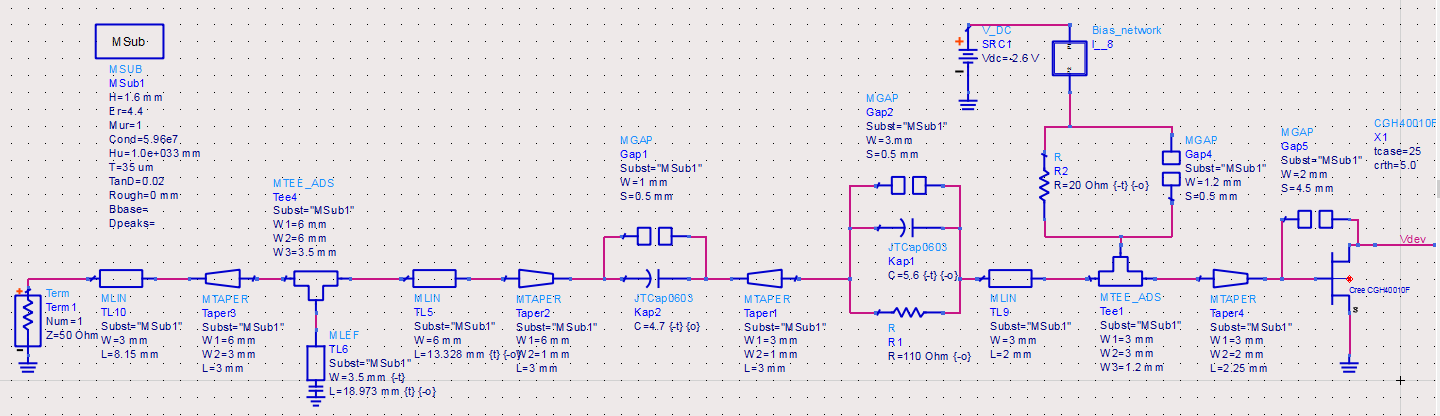
\includegraphics[width=\textwidth]{img/Circuit_input}
	  \caption{Input portion of amplifier circuit with S-parameter terminal}
	  \label{fig:Schem_Input}
  \end{figure}

  \begin{figure}[H]
	  \centering
	  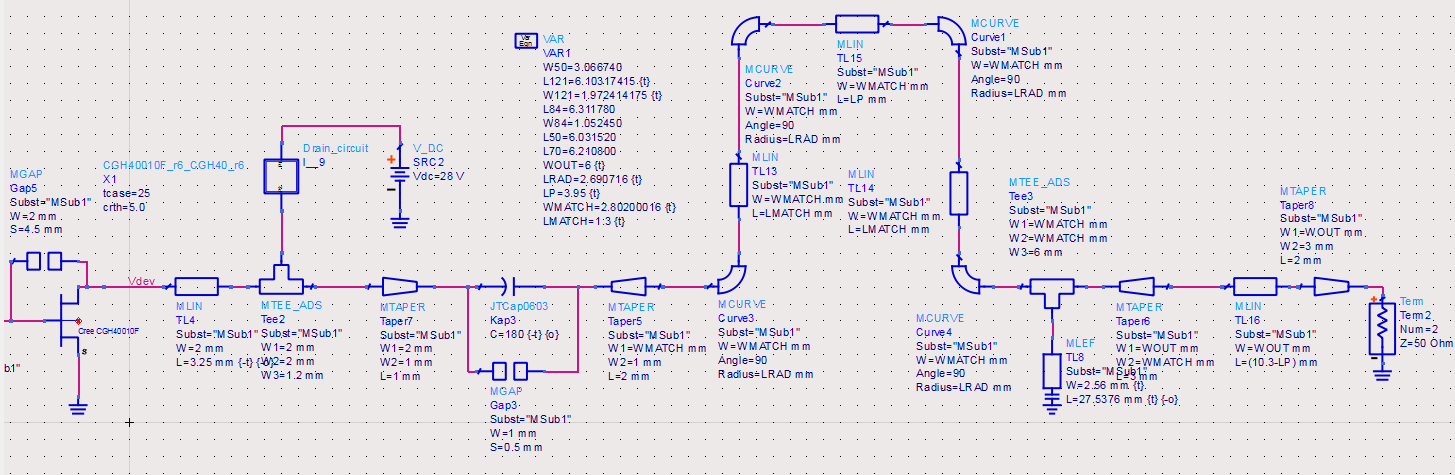
\includegraphics[width=\textwidth]{img/Circuit_output}
	  \caption{Output portion of amplifier circuit with S-parameter terminal}
	  \label{fig:Schem_Output}
  \end{figure}

  
  \begin{figure}[h]
	  \centering
	  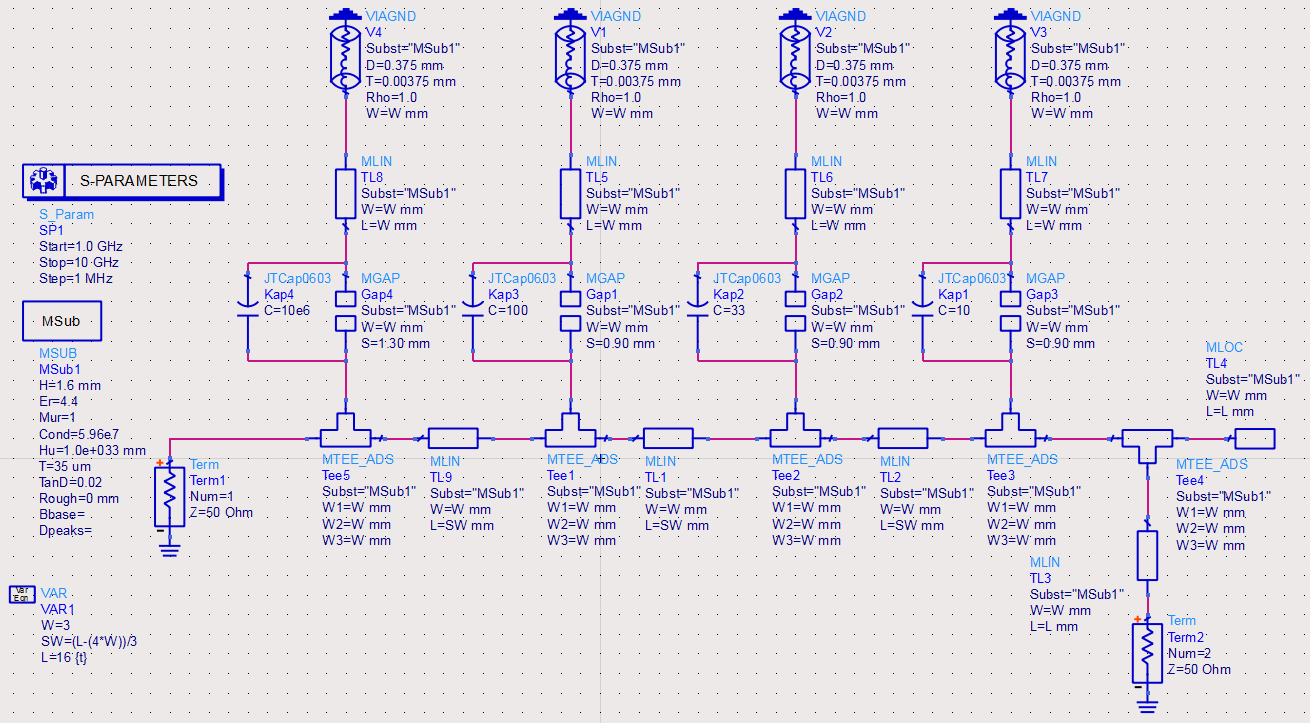
\includegraphics[width=\textwidth]{img/Bias_filter_two_port}
	  \caption{Schematics of input and output bias network}
	  \label{fig:Schem_Bias}
  \end{figure}

  \begin{figure}[h]
	  \centering
	  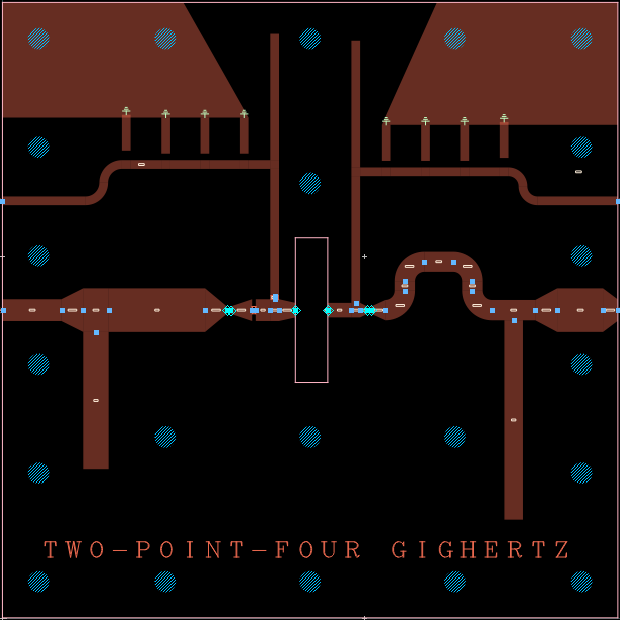
\includegraphics[width=0.75\textwidth]{img/Layout_ads}
	  \caption{PCB layout}
	  \label{fig:Layout}
  \end{figure}



\chapter{Additional graphs}

  \begin{figure}[h]
	  \centering
	  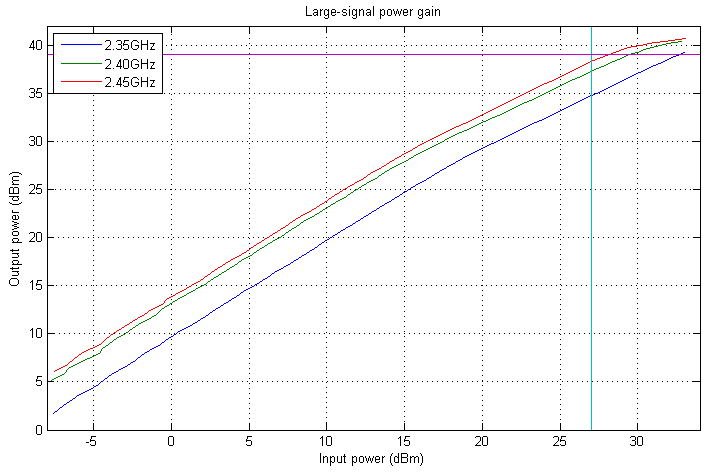
\includegraphics[width=0.75\textwidth]{img/Power_Out_1tone}
	  \caption{Measured output power at three different frequencies}
	  \label{fig:Meas_Pout}
  \end{figure}

  \begin{figure}[H]
	  \centering
	  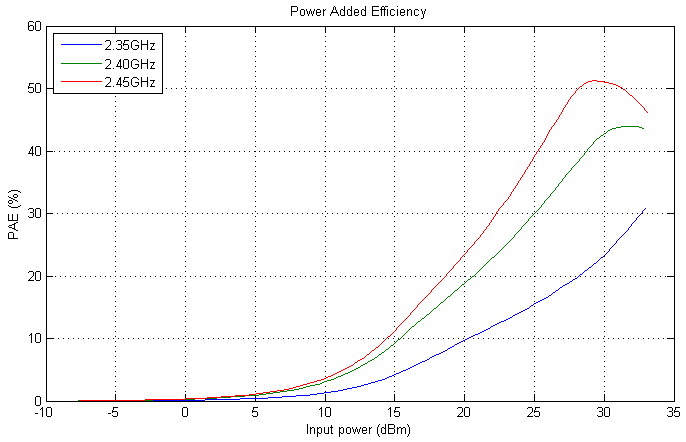
\includegraphics[width=0.75\textwidth]{img/Power_Added_Efficiency}
	  \caption{Measured power added efficiency at three different frequencies}
	  \label{fig:Meas_Pae}
  \end{figure}

